\documentclass[10pt,a4paper]{article}
\usepackage{rpgcover}
\usepackage{illustrated-panel}
\usepackage{longtable,booktabs}
\usepackage{float}
\usepackage{multicol}
\usepackage{fancyvrb}
\usepackage{wrapfig}
\usepackage{needspace}
\usepackage{titlesec}
\babelprovide[import]{ngerman}
\titleformat{\subsection}{\normalfont\Large\bfseries\color{rpgbrown}}{}{0pt}{}
\titlespacing*{\subsection}{0pt}{12pt plus 2pt}{5pt}
\titleformat{\subsubsection}{\normalfont\normalsize\bfseries\color{rpgbrown}}{}{0pt}{}
\titlespacing*{\subsubsection}{0pt}{10pt plus 2pt}{4pt}
\usepackage{etoolbox}
% Stat boxes never start in the last lines of a page, where they would split after their title.
\BeforeBeginEnvironment{rpgnote}{\par\needspace{8\baselineskip}}
\pretocmd{\subsection}{\needspace{5\baselineskip}}{}{}
\pretocmd{\subsubsection}{\needspace{4\baselineskip}}{}{}
\setcounter{tocdepth}{1}
\clubpenalty=10000
\widowpenalty=10000
\displaywidowpenalty=10000
\interlinepenalty=0
\emergencystretch=1.2em
\newcommand{\HHInlineFigure}[3]{%
  \begin{center}\includegraphics[width=#2\linewidth,height=56mm,keepaspectratio]{assets/hollow-hearth/#1.jpg}%
  \par\vspace{2pt}{\footnotesize\itshape\color{rpgbrown}#3\par}\end{center}}
% Scene-opening illustrations float: here when they fit, otherwise at the foot of the next page.
% They never narrow a read-aloud box or leave a gap at the bottom of a page.
\newcommand{\HHSceneArt}[2]{%
  \begin{figure}[!hb]\centering\includegraphics[width=.62\linewidth,height=58mm,keepaspectratio]{assets/hollow-hearth/#1.jpg}%
  \par\vspace{2pt}{\footnotesize\itshape\color{rpgbrown}#2\par}\end{figure}}
% Full-page maps float to the next free page instead of ending the current page early.
\newcommand{\HHSceneMap}[3]{%
  \begin{figure}[p]\centering
    {\Large\bfseries\color{rpgbrown}#2\par}\vspace{6mm}%
    \includegraphics[width=.96\linewidth,height=190mm,keepaspectratio]{assets/hollow-hearth/#1.jpg}\par\vspace{4mm}%
    {\small\itshape\color{rpgbrown}#3\par}%
  \end{figure}}
\newcommand{\HHContents}{%
  \clearpage\thispagestyle{rpg}
  \vspace*{10mm}\begin{center}{\fontsize{27}{31}\selectfont\bfseries INHALT\par}\vspace{9pt}
  {\color{rpgline}\rule{.76\linewidth}{.55pt}}\end{center}\vspace{9mm}
  \begingroup
  \expandafter\def\csname l@section\endcsname##1##2{\csname @dottedtocline\endcsname{1}{0em}{4em}{\bfseries ##1}{##2}}%
  \csname @starttoc\endcsname{toc}\endgroup
  \vspace{5mm}
  \begin{center}
\includegraphics[height=68mm,width=.59\linewidth,keepaspectratio]{assets/hollow-hearth/front-overlay.png}\end{center}
  \vfill
  \begin{center}{\small\itshape Ein Abenteuer von Jacopo Biscella\par}\vspace{5pt}
  {\footnotesize Dieses Abenteuer steht wie Der letzte Wurf unter der Lizenz Creative Commons Namensnennung–Weitergabe unter gleichen Bedingungen 4.0 International (CC BY-SA 4.0). Weitergabe und Bearbeitung, auch kommerziell, sind erlaubt, wenn der Autor genannt wird und abgeleitete Werke gleich lizenziert bleiben.\par}\end{center}
  \clearpage}
\RPGSetRunningTitle{Die Glocke von Hohlherd}
\RPGSetCoverWordSpace{.78em}
\hypersetup{pdftitle={Die Glocke von Hohlherd},pdfauthor={Jacopo Biscella}}
\setlength{\emergencystretch}{2em}
\setcounter{secnumdepth}{-1}
\newcommand{\tightlist}{\setlength{\itemsep}{0pt}\setlength{\parskip}{0pt}}

\newcommand{\HHFrontArt}{assets/hollow-hearth/front-overlay.png}
\newcommand{\HHBackArt}{assets/hollow-hearth/back-overlay.png}
% Existing rpgcover.sty is used unchanged; only an adventure-specific back-cover layout follows.

\let\HHUnchangedChapter\RPGChapter
\renewcommand{\RPGChapter}[1]{\par\needspace{12\baselineskip}\HHUnchangedChapter{#1}}

\setlength{\parskip}{3pt plus .5pt minus .5pt}
\linespread{1.06}\selectfont
\newcommand{\HHAdventureBackCover}{%
 \clearpage\pagenumbering{gobble}\RPGCoverPagetrue\thispagestyle{empty}\null
 \begin{tikzpicture}[remember picture,overlay,x=1mm,y=1mm]
  \RPGDrawBackground{\RPGBackBackgroundFile}
  \node[align=center,text=coverink,text width=170mm,inner sep=0pt] at ($(current page.south west)+(105mm,260mm)$)
    {{\RPGCoverTitleFont\fontsize{19}{23}\selectfont DIE GLOCKE VON HOHLHERD}};
  \draw[coverink,line width=.45pt] ($(current page.south west)+(57mm,246mm)$)--($(current page.south west)+(153mm,246mm)$);
  \node[anchor=north,align=left,text=coverink,text width=137mm,inner sep=0pt] at ($(current page.south west)+(105mm,240mm)$)
    {\RPGCoverTextFont\fontsize{10.4}{13.4}\selectfont
    Vor sieben Generationen segnete ein wandernder Mystiker eine Bronzeglocke. Das Dorf am Ende der Königsstraße, wo der Wald beginnt, wurde Hohlherd genannt. Jeden Abend hielt die Glocke das Hohle Volk fern, blasse rindenhäutige Wesen, die zwischen den Bäumen flüstern.};
  \node[anchor=north,align=center,text=coverink,text width=140mm,inner sep=0pt] at ($(current page.south west)+(105mm,197mm)$)
    {\RPGCoverSubtitleFont\fontsize{13}{17}\selectfont Vor drei Nächten wurde die Glocke gestohlen.\\[4pt]
    Die nächste mondlose Nacht kommt in achtundvierzig Stunden.};
  \draw[coverink,line width=.45pt] ($(current page.south west)+(57mm,167mm)$)--($(current page.south west)+(153mm,167mm)$);
  \node[anchor=north,align=left,text=coverink,text width=137mm,inner sep=0pt] at ($(current page.south west)+(105mm,162mm)$)
    {\RPGCoverTextFont\fontsize{9.9}{12.1}\selectfont
    Ein Einführungsabenteuer für Der letzte Wurf, für drei oder vier Protagonisten und eine Sitzung von zwei bis drei Stunden. Es vermittelt Würfelstufen, erzählerische Entfernungen, Wunden, Ermüdung, Magie und Rückschläge.};
  \node[anchor=north,align=center,text=coverink,text width=147mm,inner sep=0pt] at ($(current page.south west)+(105mm,133mm)$)
    {\RPGCoverSubtitleFont\fontsize{10.5}{13.2}\selectfont
     Drei Wege. Ein Ende nach dem Willen der Gruppe.\\
     Ein entehrter Ritter. Ein rätselhafter Käufer.\\
     Eine Entscheidung für alle.};
  \node[anchor=north,align=center,text=coverink,text width=144mm,inner sep=0pt] at ($(current page.south west)+(105mm,114mm)$)
    {\RPGCoverTextFont\fontsize{10.2}{12.5}\selectfont
     Enthält: vier Karten $\cdot$ fünf Illustrationen $\cdot$\\ eine Schnellreferenz für den Erzähler.};
  \RPGOptionalArtwork{105}{59}{130}{24}{\HHBackArt}
  \filldraw[fill=white,draw=coverink,line width=.55pt]
    ($(current page.south west)+(139mm,25mm)$) rectangle
    ($(current page.south west)+(187mm,55mm)$);
 \end{tikzpicture}
 \clearpage\RPGCoverPagefalse
}
\newcommand{\HHFrontCover}{%
 \clearpage\RPGCoverPagetrue\thispagestyle{empty}\null
 \begin{tikzpicture}[remember picture,overlay,x=1mm,y=1mm]
  \RPGDrawBackground{\RPGFrontBackgroundFile}
  \node[align=center,text=coverink,text width=138mm,inner sep=0pt]
   at ($(current page.south west)+(105mm,248mm)$)
   {\RPGCoverTitleFont\fontsize{16.6}{20.7}\selectfont DIE GLOCKE VON\\[1.0mm]HOHLHERD};
  \node[align=center,text=coverink,text width=135mm,inner sep=0pt]
   at ($(current page.south west)+(105mm,235mm)$)
   {\RPGCoverSubtitleFont\fontsize{9.0}{11.6}\selectfont Ein Abenteuer zu »Der letzte Wurf«};
  \RPGOptionalArtwork{105}{119}{150}{138}{\HHFrontArt}
  \node[align=center,text=coverink,text width=124mm,inner sep=0pt]
   at ($(current page.south west)+(105mm,25mm)$)
   {\RPGCoverTextFont\fontsize{12}{15}\selectfont Jacopo Biscella};
 \end{tikzpicture}\clearpage\RPGCoverPagefalse}
\begin{document}
% Select the language here: babel resets to its main language (english) at \begin{document}.
\selectlanguage{ngerman}
\RPGStartFrontMatter
\HHFrontCover
\HHContents
\RPGStartMainMatter
\RPGChapter{Die Glocke von Hohlherd}
\begin{center}\textit{Ein Einführungsabenteuer für Der letzte Wurf}\par\smallskip
\small 2--3 Stunden \textperiodcentered\ 3--4 Protagonisten \textperiodcentered\ Mindestens ein Kämpfer \textperiodcentered\ Ausgabe für den Erzähler
\end{center}
\noindent\textit{Die vier vorgefertigten Protagonisten stehen bei den Downloads dieses Abenteuers bereit: ein PDF pro Charakterbogen, nach der Charakterbogenvorlage des Regelbuchs.}\par\medskip
\subsection{Ein Wort an den Erzähler}\label{ein-wort-an-den-erzuxe4hler}

Dieses Abenteuer ist zuerst ein Lehrstück und erst dann eine Geschichte. Jede Szene rückt einen bestimmten Grundpfeiler von \emph{Der letzte Wurf} in den Vordergrund, ohne die Handlung je für eine Regelerklärung anzuhalten. Wenn der Abspann läuft, haben deine Spieler Würfe auf verschiedenen Stufen, erzählerische Entfernungen, den gemeinsamen Vorrat aus Wunden und Ermüdung, die Hilfe-Regel und -- wenn du deine Sache gut machst -- mindestens eine Verausgabung erlebt, mit zitternder Hand erklärt, genau in dem Augenblick, den der Titel verspricht.

Als Zeitplan gilt ungefähr:

\begin{itemize}
\tightlist
\item
  30 Minuten für Charaktererschaffung und Vorbereitung \emph{(nach den Erschaffungsregeln im Regelbuch, S. 2--6)}
\item
  35 Minuten für \textbf{Szene 1 · Das Dorf} (soziale Untersuchung)
\item
  40 Minuten für \textbf{Szene 2 · Der Flüsterwald} (Fertigkeitsprobe und Atmosphäre)
\item
  60 Minuten für \textbf{Szene 3 · Der alte Wachturm} (Kampf als Höhepunkt und Auflösung)
\item
  10 Minuten für \textbf{Die drei Fragen} und die Folgen
\end{itemize}

Eine Erinnerung, die man nicht oft genug wiederholen kann: In diesem Spiel gibt es keine Initiativewürfe, keine feste Zugreihenfolge und kein Raster. Die Karten in diesem Abenteuer sind räumliche Anker für die Vorstellungskraft aller am Tisch -- Entfernungen sind am Spieltisch immer \textbf{Direkt}, \textbf{Nah}, \textbf{In Reichweite} oder \textbf{Fern}.

\par\vspace{3pt}

\subsection{Was dieses Abenteuer vermittelt}\label{was-dieses-abenteuer-vermittelt}

\begingroup\setlength{\arrayrulewidth}{.34pt}\arrayrulecolor{rpgline}\renewcommand{\arraystretch}{1.32}\rowcolors{2}{rpgshade}{white}\par\smallskip\noindent\begin{tabularx}{\linewidth}{|Y|Y}\hline
\rpghead{Szene} & \rpghead{Eingeführte Regeln} \\ \hline
Das Dorf & Würfe auf Attribut + Fertigkeit; ZW für soziale Handlungen; Vergleichswürfe; Merkmal und Bürde ins Spiel bringen \\ \hline
Der Flüsterwald & Hilfe; Zustände ($-1$ Stufe); erzählerische Entfernungsstufen \\ \hline
Der alte Wachturm & Kampf; Wunden und Ermüdung; kritischer Erfolg; Rückschlag; \textbf{Verausgabung}; Folgen \\ \hline
\end{tabularx}\arrayrulecolor{black}\endgroup\par\smallskip

Gehört ein Mystiker zur Gruppe, wird in Szene 3 wahrscheinlich auch sein erster Rückschlag eintreten -- lass es zu.

\par\vspace{3pt}

\par\needspace{65mm}\subsection{Die Ausgangslage}\label{die-ausgangslage}

\begin{wrapfigure}{r}{.38\linewidth}\vspace{-5pt}\centering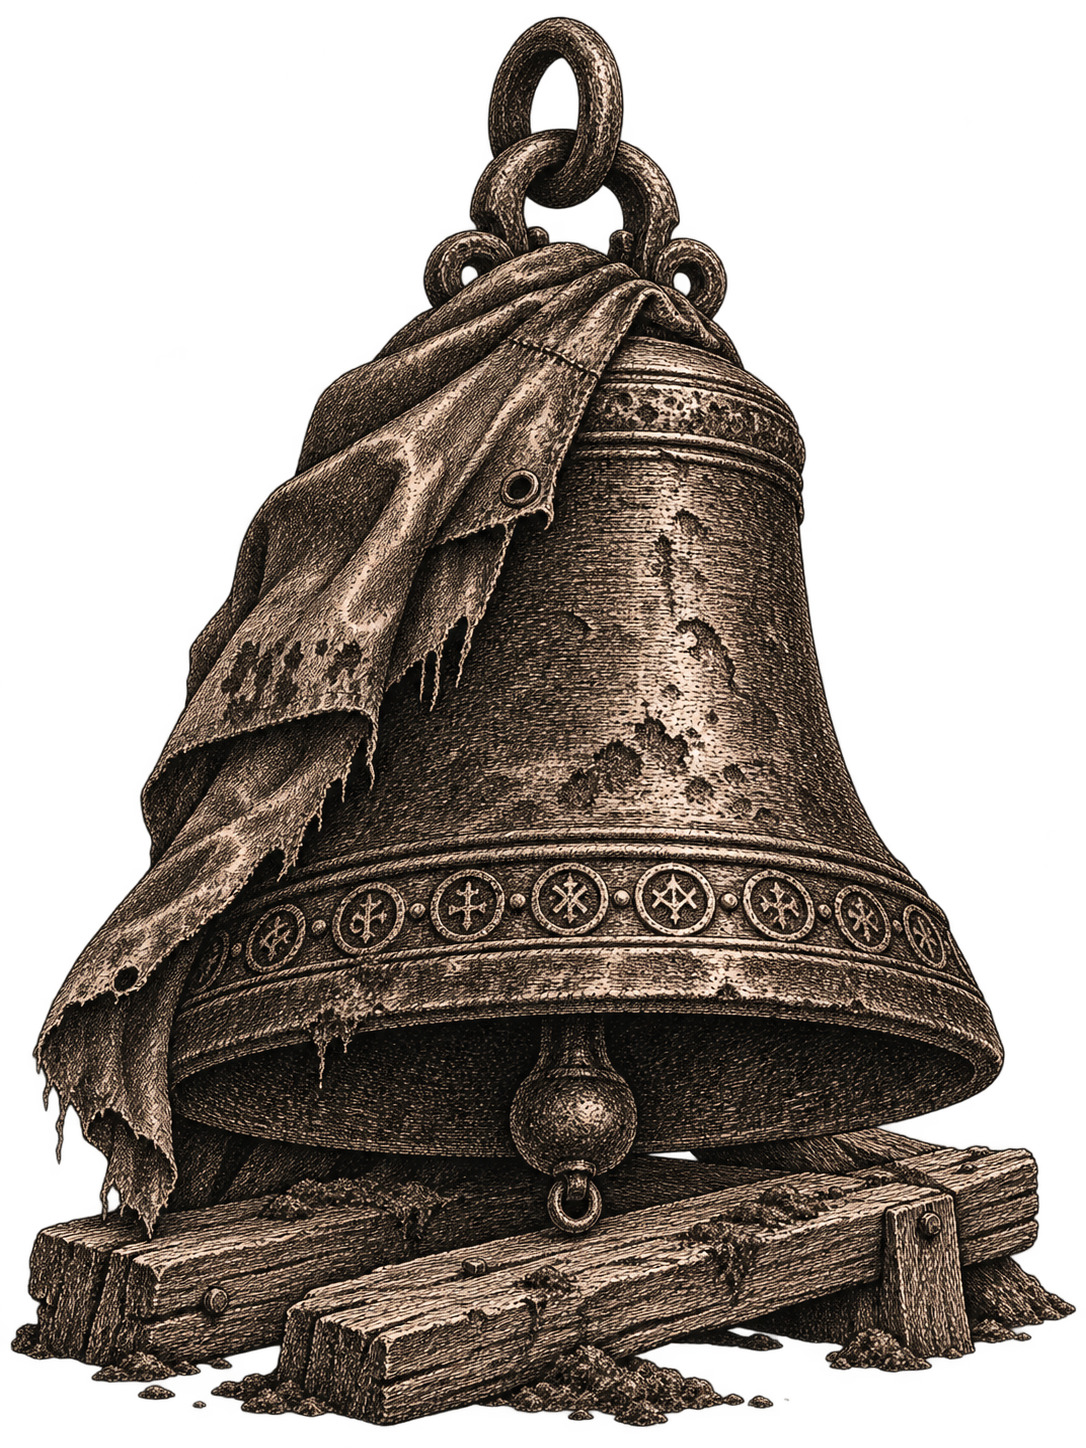
\includegraphics[width=.98\linewidth,height=58mm,keepaspectratio]{assets/hollow-hearth/bell.jpg}\par{\scriptsize\itshape\color{rpgbrown}Die gestohlene Glocke, in Wachstuch gewickelt}\vspace{-5pt}\end{wrapfigure}

Vor sieben Generationen segnete ein wandernder Mystiker namens \textbf{Veyl Ashen} eine Bronzeglocke, gegossen in der Schmiede einer kleinen Siedlung dort, wo die Königsstraße endet und der alte Wald beginnt. Die Siedlung erhielt den Namen \textbf{Hohlherd}. Die Glocke, die bei jeder Abenddämmerung geläutet wurde, hielt das \textbf{Hohle Volk} -- blasse, rindenhäutige Wesen, die zwischen den Bäumen hervor flüstern -- unten bei den Wurzeln, wo es hingehört.

Vor drei Nächten wurde die Glocke gestohlen.

Eine Räuberbande unter einem Deserteur namens \emph{»Sir«} \textbf{Corwin Vask} kam aus den Ruinen des Wachturms herab, in denen sie lagert, tötete den Lehrling des alten Glöckners und verschwand mit der in Wachstuch gewickelten Glocke nach Norden in den Wald. Gestern Morgen haben die Dorfbewohner den Jungen begraben.

Die nächste mondlose Nacht ist in \textbf{achtundvierzig Stunden}.

Das ist die Frist. Wenn in jener Nacht der Mond untergegangen ist und in der Dämmerung keine Glocke geläutet hat, kehrt das Hohle Volk nach Hohlherd zurück -- in ein Dorf, das vergessen hat, wie man sich verteidigt.

\par\vspace{3pt}

\subsection{Der Einstieg}\label{der-einstieg}

\HHSceneArt{village}{Hohlherd in der Dämmerung: das leere Podest}

Passe die Ankunft an die Merkmale und Bürden an, die deine Spieler aufgeschrieben haben. Ein paar schnelle Anregungen:

\begin{itemize}
\tightlist
\item
  Ein \textbf{Gelehrter}, der in alten liturgischen Aufzeichnungen der Abstammung von Veyl Ashen nachspürt.
\item
  Ein \textbf{Abenteurer} mit einem Auftrag aus dem nächsten Ort weiter oben an der Straße.
\item
  Ein \textbf{Mystiker}, der meilenweit entfernt \emph{gespürt} hat, wie die Glocke verstummte.
\item
  Ein \textbf{Kämpfer}, der einem Schlachtfeld den Rücken kehrt, auf dem er nicht länger stehen will.
\end{itemize}

Wie sie auch kommen: Die Dorfvorsteherin \textbf{Hesta Thrush} bietet ihnen das Wenige, das Hohlherd besitzt -- Münzen, Gastfreundschaft und ein seit der Gründung gehütetes Relikt (siehe \emph{Auflösung}) --, wenn sie die Glocke heimbringen.

\begin{quote}
\subsubsection{Zum Vorlesen --- Die Ankunft}\label{zum-vorlesen-die-ankunft}

\emph{Die Straße wird zum Weg, der Weg zum Fußpfad, und der Fußpfad mündet in eine Lichtung mit niedrigen Steinhäusern unter steilen Schieferdächern. Mitten auf dem Dorfplatz steht ein hölzernes Podest. Leer. Vier eiserne Bolzen, wo etwas Schweres herausgerissen wurde. Aus den Schornsteinen steigt kein Rauch. Auf dem Platz ist niemand.}

\emph{Dann öffnet sich eine Tür, eine alte Frau tritt heraus, und hinter ihr hört ihr jemanden weinen.}
\end{quote}

\par\vspace{3pt}

\HHSceneMap{map-village}{Hohlherd: Anlage des Dorfes}{Das Glockenpodest steht auf dem Dorfplatz; Hesta, Bram, Vela und die Schenke sind in der Nähe. Alle Orte im Dorf: Nah.}
\RPGChapter{Szene 1 — Das Dorf}\label{szene-1-das-dorf}

\textbf{Regelschwerpunkt:} Wissenswürfe, Fertigkeitsboni, Vergleichswürfe, Merkmal und Bürde ins Spiel bringen.

Drei Menschen in Hohlherd sind für eure Nachforschungen wichtig. Die Protagonisten können mit allen dreien sprechen, in beliebiger Reihenfolge. Jeder besitzt ein Stück des Gesamtbilds, und mindestens einer von ihnen lügt \emph{beinahe}.

\par\smallskip\begin{rpgnote}[fontupper=\normalfont]\textbf{NSC im Dorf}\par\smallskip
\textbf{Hesta Thrush} \emph{(NSC)} -- Wissen Kompetent. Keine Kampfwerte; wenn Gewalt sie trifft, ist sie genau das, was sie zu sein scheint.\par\smallskip
\textbf{Vela Roan} \emph{(NSC)} -- Wissen Experte (Kräuterkunde, Überleben), Wunder Kompetent. Kämpft nur, wenn sie in die Enge getrieben wird.\par\smallskip
\textbf{Der alte Bram} \emph{(NSC)} -- Wissen Kompetent. Kann nicht mehr kämpfen.\end{rpgnote}\par\smallskip
Die Anlage zeigt \textbf{die Dorfkarte von Hohlherd}. Alle Orte im Dorf liegen in der Entfernung \textbf{Nah} zueinander.

\subsubsection{Hesta Thrush --- Die Dorfvorsteherin}\label{hesta-thrush-die-dorfvorsteherin}

Eine Frau um die sechzig, vom Wetter gegerbt, von Trauer schmal geworden. Ihr Sohn zog in den Krieg und kam nie zurück; seit elf Jahren ist sie Dorfvorsteherin und kennt jeden im Dorf beim zweiten Vornamen.

Was sie bereitwillig erzählt:

\begin{itemize}
\tightlist
\item
  Die Räuber kamen aus dem \textbf{alten Wachturm}, vier Stunden Fußmarsch nördlich im Flüsterwald.
\item
  Als letzte Belohnung des Dorfes bietet sie ein Relikt aus der Gründungszeit an: die \textbf{Salzklinge} \emph{(Regelbuch, S. 10)}.
\end{itemize}

Worüber sie lügen wird:

Sie weiß, dass ihr Cousin \textbf{Marrel} in der Woche vor dem Diebstahl in der Schenke mit einem der Räuber beim Trinken gesehen wurde. Sie will nicht, dass ihr Cousin dafür gehängt wird. Ein \textbf{Wissenswurf als Vergleichswurf gegen Hestas Wissen (Kompetent)} bemerkt ihr Unbehagen. \textbf{Diplomatie} bringt sie dazu, mit der Wahrheit herauszurücken; \textbf{Rhetorik} ebenso. \textbf{Einschüchtern, ZW 5} funktioniert auch, bringt aber das Dorf für den Rest des Abenteuers gegen die Gruppe auf.

\begin{quote}
\subsubsection{Ansatz für Merkmal und Bürde}\label{ansatz-fuxfcr-wesenszug-und-buxfcrde}

Ein Protagonist, dessen Bürde mit Krieg, verlorenen Kindern oder gebrochenen Eiden zu tun hat, findet in Hesta entweder eine Verbündete oder einen Spiegel. Spiel das aus. \emph{»Du erinnerst mich an ihn«}, sagt sie und sieht dabei die falsche Person an.
\end{quote}

\subsubsection{Der alte Bram --- Der Glöckner}\label{der-alte-bram-der-gluxf6ckner}

Der Glöckner, über achtzig, hat nur überlebt, weil er sich gerade in den Brombeeren erleichterte, als die Räuber kamen. Der getötete Junge war sein Lehrling und sein Großneffe. Er ist wütend. Nicht laut. Auf die andere Art.

Was er gesehen hat:

\begin{itemize}
\tightlist
\item
  Vier Männer. Einer in Rüstung, einer mit Langbogen, zwei mit Dolchen.
\item
  Der Gerüstete trug \textbf{eine weiße Sonne auf der Schulter seines Umhangs} -- das Wappen eines Ritterordens, der vor zehn Jahren in Ungnade fiel. Ein \textbf{Wissenswurf, ZW 4 mit der Fertigkeit Geschichte}, erkennt den Orden als den \textbf{Orden der Blassen Sonne}, der in den Kriegen wegen »ritueller Vergehen« aufgelöst wurde. Ohne Geschichte braucht es \textbf{ZW 5}, um eine vage Erinnerung hervorzukramen.
\item
  Er glaubt, dass die Glocke lebt. Vielleicht hat er recht.
\end{itemize}

\subsubsection{Vela Roan --- Die Kräuterkundige}\label{vela-roan-die-kruxe4uterkundige}

Vierzig, scharfsinnig, die Einzige im Dorf, die \emph{in} den Flüsterwald gegangen und zurückgekommen ist. Sie weiß, was das Hohle Volk ist. Sie wird es nicht offen sagen. Sie spricht in Geschichten.

Was sie anbietet, wenn man sie richtig fragt:

\begin{itemize}
\tightlist
\item
  Die »Rindenleute« kommen aus den Wurzeln, wenn keine Glocke läutet. Sie glaubt, dass bereits ein Wesen des Hohlen Volks in Menschengestalt unter den Dorfbewohnern wandelt.
\item
  Sie gibt ein Fläschchen \textbf{destillierte Nachtwurzel} -- \emph{ein besonderer Gegenstand: Auf eine Klinge gegossen, verursacht der nächste Treffer gegen unnatürliche Wesen +1 Wunde; nur eine Anwendung} --, \textbf{wenn} ein Protagonist zusagt, ihr einen Zweig \textbf{Mondsilberblume} aus der Tiefe des Waldes mitzubringen.
\end{itemize}

Das ist eine Nebenversuchung: Gelegenheit für einen Bürde-Moment, falls später jemand sein Wort bricht, oder dafür, ein ehrenhaftes Merkmal auf die Probe zu stellen. Die Blume gibt es wirklich. Ob die Gruppe Zeit dafür findet, liegt bei ihr.

\subsubsection{Optional · Marrel, der Cousin}\label{optional-marrel-der-cousin}

Gehen die Protagonisten Hestas Lüge nach, finden sie Marrel in der Schenke, wo er gegen seine Angst antrinkt. Er bestätigt, dass der Räuber, mit dem er sprach -- ein Mann namens \textbf{Thessik} --, mit einem Käufer geprahlt hat, der \emph{»in Nordsilber bezahlt«} und die Glocke holen kommt. Marrel wusste nicht, dass sie gestohlen werden sollte. \textbf{Einschüchtern, ZW 4} bricht ihn. \textbf{Diplomatie, ZW 4} mit einem ausgegebenen Getränk funktioniert ebenfalls. \textbf{Handel, ZW 4}, wenn ein Gelehrter durchsprechen will, was »Nordsilber« eigentlich bedeutet (ein Ausdruck der Schmuggler, die über die Grenze gehen -- Nordsilber gibt es nicht, es ist ein Deckwort für Feengold).

\subsubsection{Hinweis für den Erzähler}\label{hinweis-fuxfcr-den-erzuxe4hler}

Wenn ein Spieler erklärt: \emph{»Ich will wissen, ob sie lügt«}, frage ihn, \textbf{wie}. Setzt er sie unter Druck? Beobachtet er sie? Ertappt er sie bei einem Widerspruch? Das \emph{Wie} bestimmt Attribut und Fertigkeit. \textbf{Wissen} ist der Normalfall, um einen Menschen zu durchschauen; \textbf{Etikette} ertappt sie bei Verstößen gegen höfische Umgangsformen, \textbf{Einschüchtern} treibt sie in Fehler, mit \textbf{Täuschung} lügst du sie in die Enge. Es gibt kein eigenes Subsystem für soziale Konflikte. Es gibt nur Wissen plus eine passende Fertigkeit gegen einen ZW. Wie bei allem anderen auch.

\par\vspace{3pt}

\HHSceneMap{map-forest}{Durch den Flüsterwald}{Unten das Dorf, oben der Turm; das Hohle Volk erscheint an dem Ufer, das die Gruppe gerade verlassen hat.}

\RPGChapter{Szene 2 — Der Flüsterwald}\label{szene-2-der-fluxfcsterwald}

\HHSceneArt{hollow}{Ein Beobachter zwischen den Bäumen}

\textbf{Regelschwerpunkt:} Hilfe, Entfernungsstufen, Zustände als $-1$ Stufe.

Ein Pfad aus zertretenem Farn und verlorenen Wachstuchfetzen führt vom Dorf nach Norden. Nach fünfzig Schritten verschluckt ihn der Flüsterwald. Die Bäume neigen sich hier nach innen.

\begin{quote}
\subsubsection{Zum Vorlesen --- Der Weg in den Wald}\label{zum-vorlesen-im-wald}

\emph{Sobald ihr den Waldrand überschreitet, sinkt das Licht um ein Drittel. Nicht wegen des Blätterdachs -- ein Blätterdach, das den Namen verdient, gibt es hier nicht --, sondern als würde die Luft selbst es trinken. Geräusche werden flach. Schritte tragen nicht mehr. Nach zehn Minuten Fußmarsch hört ihr nur noch euren eigenen Atem und, sehr weit entfernt, etwas, das Wind in den Zweigen sein könnte -- oder Stimmen, die etwas sagen, das ihr nicht ganz versteht.}
\end{quote}

Den Weg vom Dorf zum Wachturm zeigt \textbf{die Karte des Flüsterwalds}, mit der Brücke und dem Ort der Sichtung.

\subsubsection{Die Spur · Eine Überlebensprobe}\label{die-spur-eine-uxfcberlebensprobe}

Die Spur ist echt, aber leicht zu verlieren. Ein Charakter mit \textbf{Überleben} würfelt \textbf{Geschick gegen ZW 4}. Ein Charakter mit Geschick Kompetent und der Fertigkeit würfelt 2W6 und behält den höheren; mit Geschick Experte ohne die Fertigkeit würfelt er genauso; mit Geschick Ungeübt und ohne Fertigkeit würfelt er 2W6 und behält den niedrigeren, was wenig freundlich ist.

Das ist der perfekte Moment, um die \textbf{Hilfe} einzuführen \emph{(Regelbuch, S. 7)}:

\begin{itemize}
\tightlist
\item
  Ein \textbf{kompetenter Helfer} -- einer, dessen eigener Wurf bei derselben Aufgabe auf Stufe Experte oder höher läge -- gibt dem Würfelpool des Hauptakteurs \textbf{+1W6}, ohne Nachteil.
\item
  Ein \textbf{inkompetenter Helfer} -- jeder, der bei derselben Aufgabe unter der Stufe Experte würfeln würde -- gibt ebenfalls \textbf{+1W6}, \emph{erhöht aber den ZW um 1}. Ein Kämpfer, der dem Abenteurer lautstark beim Spurenlesen »hilft«, kann die Sache verschlimmern.
\end{itemize}

Lass die Spieler zusehen, wie das passiert. Ein Kämpfer, der dem Spurenleser hilft, macht aus ZW 4 einen ZW 5 -- und begreift die Lektion, wenn die Spur verloren geht.

Geht die Spur verloren, vergeht eine zusätzliche Stunde, und die Dämmerung erwischt die Gruppe im Wald. Von da an bis Sonnenaufgang wird jeder Wurf unter einem \textbf{Zustand: $-1$ Stufe} abgelegt.

\subsubsection{Die morsche Brücke}\label{die-morsche-bruxfccke}

Die Spur überquert eine Schlucht auf einer Brücke aus einem einzigen Baumstamm, um den sich seit zwanzig Jahren niemand gekümmert hat. Der Stamm trägt nur eine Person zugleich. Darunter geht es fünfzehn Meter tief hinab zu einem Bach zwischen Felsen.

\begin{itemize}
\tightlist
\item
  \textbf{Geschickwurf, ZW 4}, um sicher hinüberzukommen. Mit \textbf{Akrobatik} kein Problem.
\item
  Wer stürzt, erleidet \textbf{2 Wunden} (Kampfwunden -- durch die Felsen). Ein \textbf{Heilkundewurf, ZW 4}, in derselben Szene heilt 1 Wunde (2 bei einem kritischen Erfolg).
\item
  Ein als Handlauf gespanntes Seil (\textbf{Stärke + Handwerk oder + Ausdauer, ZW 3}) senkt den ZW für alle auf 3 und hebt die Folgen eines Fehlschlags auf.
\end{itemize}

Das ist auch eine leise Probe für ein Merkmal. Ein Protagonist mit dem Merkmal \emph{»Ich lasse niemanden zurück«}, der bei der eigenen Überquerung scheitert -- und dann von einem Gefährten hinübergeholfen wird --, sollte das spüren.

\subsubsection{Die Sichtung}\label{die-sichtung}

Ob die Gruppe gut oder schlecht hinüberkommt: Sobald \textbf{die letzte Person das andere Ufer erreicht}, erscheint auf der Seite, die sie gerade verlassen haben, zwischen zwei Bäumen ein \textbf{Wesen des Hohlen Volks}. Blass. Rindenhäutig. Ein wenig zu groß. Der Mund nicht ganz dort, wo ein Mund sein sollte. Es bewegt sich nicht. Es droht nicht. Es sieht ihnen nach, wie sie fortgehen. Nach dreißig Sekunden ist es verschwunden.

Das dient allein der Atmosphäre. Es gibt keinen Wurf. Lass die Spieler den Moment aushalten.

\begin{quote}
\subsubsection{Hinweis --- Entfernungen}\label{hinweis-entfernungen}

Das Wesen ist \textbf{Fern} (jenseits der Schlucht, außerhalb vernünftiger Bogenreichweite). Ein Mystiker mit einem Wahrnehmungs-Grimoire -- zum Beispiel \emph{Auge der Leere} (Regelbuch, S. 12) -- möchte vielleicht genauer hinsehen. Lass ihn. Lass ihn die Ermüdungskosten bezahlen. Zeig dem Tisch, wie ein Wunderwurf aussieht, wenn nur Wissen auf dem Spiel steht.
\end{quote}

\subsubsection{Die Wölfe · Optionale, skalierbare Begegnung}\label{die-wuxf6lfe-optionaler-kampf}

Kommt die Sitzung schnell voran und scheint die Gruppe noch zu wenig gefordert, kann ein Paar \textbf{ausgehungerter Wölfe} sie auf dem letzten Stück vor dem Wachturm überfallen. Zwei Wölfe vermitteln die Regel für \textbf{Gegnergruppen} (Regelbuch, S. 13) und lassen den Kämpfer zum ersten Mal zuschlagen. \par\smallskip\begin{rpgnote}[fontupper=\normalfont]\textbf{Ausgehungerter Wolf} \emph{(optionale Begegnung im Wald)} \emph{ZW S3/G4 · Kompetent · 2 Wunden · Biss (2Wu Stärke).} \emph{Verhalten: »Jagt den Schwächsten. Drei Nächte ohne Futter.«}\end{rpgnote}

\par\vspace{3pt}

\RPGChapter{Szene 3 — Der alte Wachturm}\label{szene-3-der-alte-wachturm}

\HHSceneArt{tower}{Der alte Wachturm in der Dämmerung}

\textbf{Regelschwerpunkt:} Kampf als Gespräch, Wunden und Ermüdung, kritischer Erfolg, Rückschlag, \textbf{Verausgabung}.

Der alte Wachturm besteht aus zwei Stockwerken verwitterten Steins auf einer flachen Anhöhe; das halbe Dach fehlt, in den Ritzen wächst Efeu. Vor dem Eingang glimmt ein Lagerfeuer. Zwei Räuber sitzen daran. Im Erdgeschoss schlafen zwei weitere. Im Obergeschoss sitzt \textbf{Sir Corwin Vask} bei der in Wachstuch gewickelten Glocke und wartet auf seinen Käufer.

Der Käufer wird \textbf{um Mitternacht} erwartet. Jetzt dämmert es.

Das Erdgeschoss und seine Zugänge zeigt \textbf{die Erdgeschosskarte des alten Wachturms}, die Anlage des Obergeschosses, in dem der Höhepunkt stattfindet, \textbf{die Obergeschosskarte des alten Wachturms}.
\HHInlineFigure{map-ground}{.68}{Alter Wachturm: Erdgeschoss -- Eingang und Lagerfeuer im Süden, eingestürzte Mauer im Westen, Treppe im Norden.}

\par\smallskip\begin{rpgnote}[fontupper=\normalfont]\textbf{Räuber}\par\smallskip \textbf{Räuber} \emph{ZW S3/G3 · Kompetent · 2 Wunden · Dolch (2Wu Geschick) oder kurzer Knüppel (1E Stärke).} \emph{Verhalten: »Feiglinge im fairen Kampf. Fliehen, wenn Corwin fällt.«} \emph{Als Gruppe: ein einziger Wurf, +1Wu für jedes Mitglied über das erste hinaus (höchstens +3). Jede Wunde gegen die Gruppe schaltet ein Mitglied aus.}\end{rpgnote}\par\smallskip
\subsubsection{Drei Wege}\label{drei-wege}

Die Gruppe hat Möglichkeiten. Frage vor dem ersten Wurf ganz direkt: \emph{»Wie wollt ihr das angehen?«} Die Regeln richten sich danach.

\textbf{Schleichen.} Die eingestürzte Mauer an der Westseite lässt sich mit einem \textbf{Wurf auf Wissen + Taktik, ZW 3}, oder durch einfache Beschreibung entdecken. Jeder Charakter würfelt \textbf{Geschick + Heimlichkeit, ZW 4}, um sich ungesehen zu nähern. Ein Fehlschlag alarmiert die beiden Räuber am Lagerfeuer. Zwei Fehlschläge alarmieren alle, auch Corwin. Eine saubere Annäherung lässt die Gruppe das Obergeschoss erreichen und ihn überraschen.

\par\Needspace{10\baselineskip}\noindent\textbf{Verhandeln.} Zum Lagerfeuer gehen und reden. Corwin ist ein Mann mit gebrochenem Stolz. Spricht ihn ein Protagonist (besonders der Kämpfer) als \emph{»Sir Corwin«} an, bekommt seine Bürde Risse. \textbf{Wissen + Diplomatie oder Rhetorik, ZW 5} bringt ihn dazu, \emph{in Erwägung zu ziehen}, die Glocke lieber zurückzuverkaufen als an den Käufer. Er wird mehr verlangen als die Belohnung des Dorfes -- aber die Gruppe kann es versprechen. Ihn über die Belohnung zu belügen ist ein \textbf{Wurf auf Wissen + Täuschung als Vergleichswurf gegen sein Wissen (Kompetent)}.

\textbf{Angriff.} Kämpfend hineingehen. Zwei Räuber am Feuer, zwei drinnen, Corwin oben. Laut, blutig und der klarste Weg, neuen Spielern den Kampf beizubringen.

\par\smallskip\begin{rpgnote}[fontupper=\normalfont]\textbf{Sir Corwin Vask, entehrter Ritter} \emph{ZW S4/G5 · Experte · 6 Wunden · Langschwert (2Wu Stärke) · schwere Rüstung.} \emph{Verhalten: »Schlägt keinen Mann, der auf den Knien liegt. Duelliert sich mit jedem, der ihn ›Sir‹ nennt. Hasst Mystiker -- sein Orden hat es ihn gelehrt.«} \emph{Optional: Er trägt ein verbeultes Medaillon mit einem Bild seiner Schwester. Sieht ein Protagonist es während des Kampfes, gib ihm die Gelegenheit, es zu nutzen.}\end{rpgnote}\par\smallskip
\subsubsection{Das Obergeschoss}\label{das-obergeschoss}

Die Glocke, Sir Corwin und die entscheidende Konfrontation befinden sich alle im Obergeschoss. Seine Anordnung ist wichtig, weil die taktischen Entscheidungen der Spieler davon abhängen.

\par\medskip\noindent
\begin{tabular}{@{}p{.60\linewidth}@{\hspace{.028\linewidth}}p{.345\linewidth}@{}}
\centering\vspace{0pt}
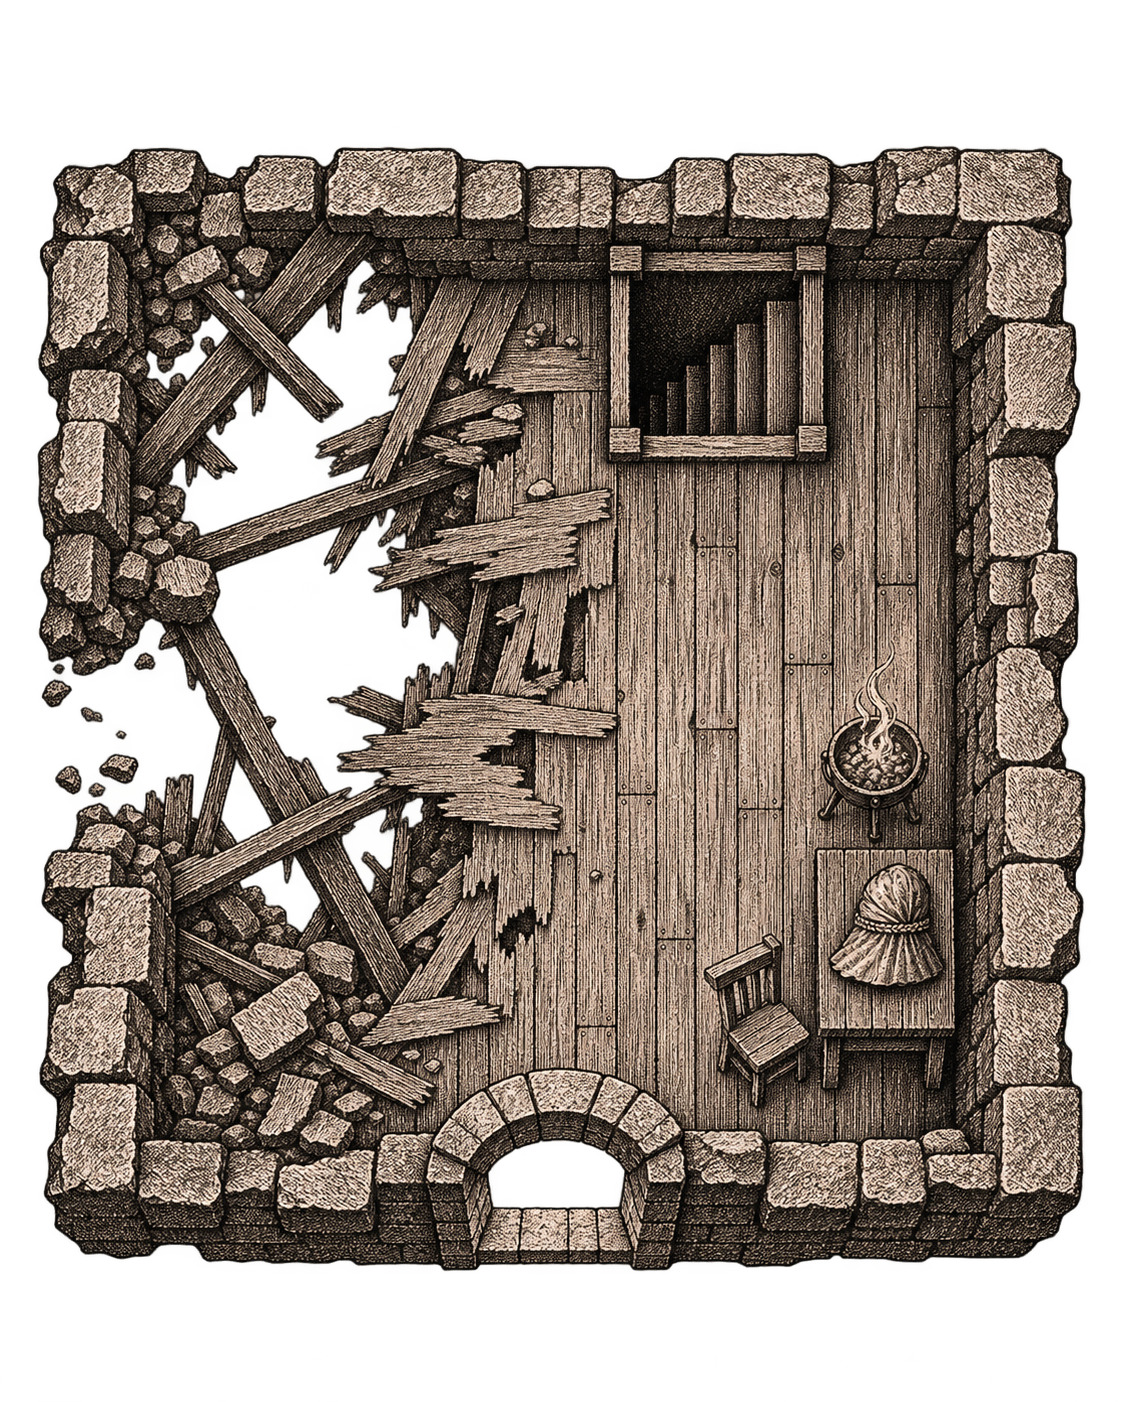
\includegraphics[width=.98\linewidth,height=70mm,keepaspectratio]{assets/hollow-hearth/map-upper.jpg}\par\vspace{2pt}
{\footnotesize\itshape\color{rpgbrown}Alter Wachturm: Obergeschoss\par}
{\scriptsize Treppe im Norden; offene Westseite; Südfenster, Glocke und Kohlebecken auf der intakten Ostseite.\par}
&
\centering\vspace{0pt}
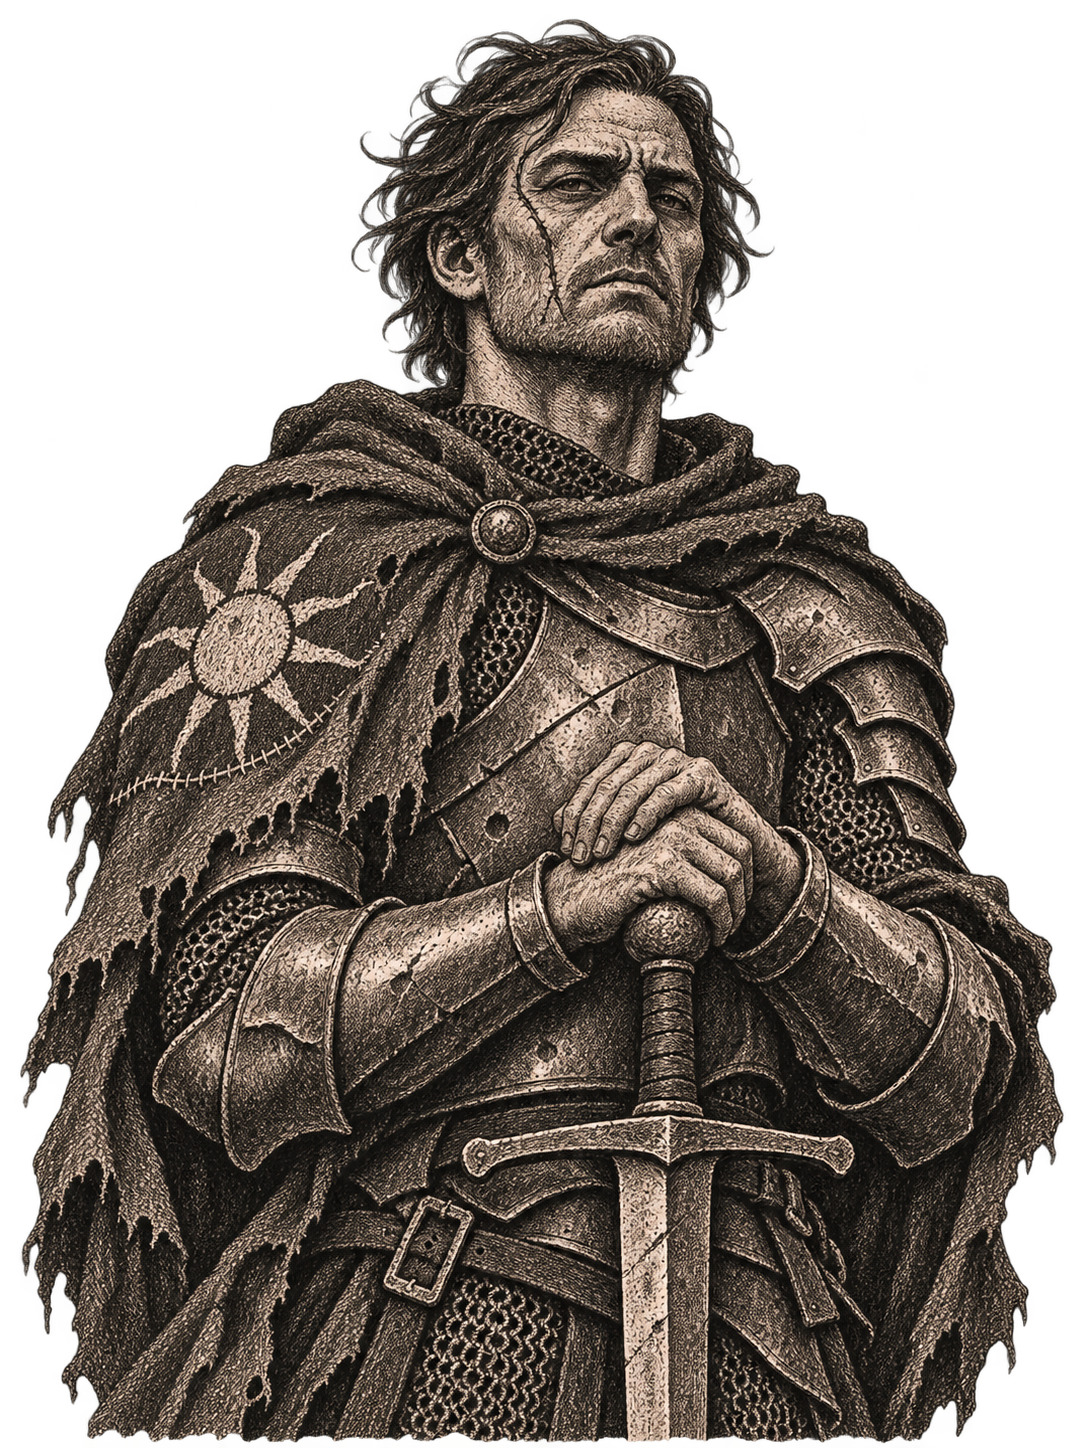
\includegraphics[width=.95\linewidth,height=68mm,keepaspectratio]{assets/hollow-hearth/corwin.jpg}\par\vspace{2pt}
{\footnotesize\itshape\color{rpgbrown}Sir Corwin Vask\par}
\end{tabular}
\par\medskip

Sir Corwin sitzt auf einem Holzstuhl neben dem \textbf{Südfenster} und beobachtet den Pfad, auf dem der Käufer heraufkommen wird. Die Glocke steht neben ihm auf einem kleinen Tisch, noch immer in schlammverschmiertes Wachstuch gehüllt. Ein Kohlebecken mit schwacher Glut spendet das einzige warme Licht im Raum. Die Treppe kommt an der Nordwand herauf -- \textbf{hinter ihm}.

Über der \textbf{westlichen Hälfte des Obergeschosses liegt offener Himmel}: Derselbe Einsturz, der im Erdgeschoss die Westmauer einriss, hat auch das westliche Dach und einen Teil des westlichen Bodens mitgenommen. Lose Balken hängen schräg herab. Den freiliegenden Westteil des Bodens kann man ohne Vorsicht nicht sicher betreten.

Dadurch entsteht ein \textbf{vierter Weg}, den der bisherige Text nur angedeutet hat:

\textbf{Das Klettern.} Ein Charakter mit \textbf{Akrobatik} kann den Schutthaufen der eingestürzten Mauer im Erdgeschoss erklimmen und an der Außenseite der zerbrochenen Westmauer weiterklettern, um durch die Lücke im Dach einzusteigen. Würfle \textbf{Geschick + Akrobatik, ZW 4}, für ein sauberes Klettern; ohne Akrobatik \textbf{ZW 5}. Ein Fehlschlag bedeutet einen Sturz -- 1 Wunde durch die Höhe und dazu der Lärm des Sturzes (Corwin hört ihn). Bei Erfolg landet der Charakter im Obergeschoss \emph{hinter} Corwin und überrascht ihn. Dieser Weg ist nur für eine einzelne Figur: Der Kämpfer in schwerer Rüstung schafft diese Kletterei nicht, und der Mystiker mit 2 LP kann sich den Sturz bei einem Fehlschlag nicht leisten. \textbf{Am besten eignet sich ein gewandter Abenteurer für diesen Weg.}

\par\Needspace{12\baselineskip}\noindent\textbf{Taktische Besonderheiten des Obergeschosses:}

\begin{itemize}
\tightlist
\item
  \textbf{Das Südfenster.} Wer die Glocke erreicht, kann sie hinauswerfen -- sie schlägt unten beim Lagerfeuer hart auf und bekommt dabei womöglich einen Sprung. Der Käufer, der vom Pfad aus zusieht, bemerkt es. Ein Protagonist kann durch das Fenster auch aus dem Raum fliehen und sich zu Boden fallen lassen (Geschick + Akrobatik, \textbf{ZW 4} für eine saubere Landung; ein Fehlschlag kostet 1 Wunde).
\item
  \textbf{Die unsichere Westhälfte.} Ein Kampf auf der eingestürzten Hälfte wird unter einem Zustand ausgetragen: \textbf{$-1$ Stufe}. Wer über die Kante gedrängt wird, stürzt ein Stockwerk tief (2 Wunden). Corwin, der den Raum kennt, kämpft nur auf der Osthälfte -- und versucht nur zu gern, Gegner auf den schlechten Boden zu drängen.
\item
  \textbf{Das Kohlebecken.} Wird es umgestoßen, verteilt sich die Glut über den trockenen Holzboden -- das Feuer breitet sich im Lauf von zwei Szenen voller Handlung aus, und der Raum wird unbewohnbar. Ein verzweifelter Zug, den jeder machen kann und der die Gruppe retten oder die Glocke mitsamt allem anderen zerstören kann.
\item
  \textbf{Sir Corwins schwere Rüstung.} Seine schwere Rüstung setzt den ZW, um ihn zu treffen, auf \textbf{4 mit Stärke} oder \textbf{5 mit Geschick}. Sie verringert den Schaden nicht. Ein umgestoßenes Kohlebecken, ein Stoß zur eingestürzten Kante hin oder ein kritischer Erfolg eines Protagonisten, der Verausgabung erklärt hat, kann die Konfrontation wenden.
\end{itemize}

\subsubsection{Die Begegnung anpassen}\label{den-kampf-anpassen}

\begingroup\setlength{\arrayrulewidth}{.34pt}\arrayrulecolor{rpgline}\renewcommand{\arraystretch}{1.32}\rowcolors{2}{rpgshade}{white}\par\smallskip\noindent\begin{tabularx}{\linewidth}{|Y|Y|Y}\hline
\rpghead{Gruppengröße} & \rpghead{Räuber} & \rpghead{Sir Corwin} \\ \hline
3 Spieler & 3 Räuber (als Gruppe) & Ja \\ \hline
4 Spieler & 4 Räuber (2 draußen, 2 drinnen) & Ja \\ \hline
\end{tabularx}\arrayrulecolor{black}\endgroup\par\smallskip

Tut sich die Gruppe sehr schwer, lass einen Räuber beim ersten Anzeichen echten Blutvergießens fliehen. Spaziert sie mühelos hindurch, trifft der Käufer früher ein.

\subsubsection{Die Wendung · Der Käufer}\label{die-wendung-der-kuxe4ufer}

Ist die Gruppe \textbf{um Mitternacht} noch am Wachturm -- ob mitten im Kampf, im Gespräch oder nach dem Sieg --, tritt eine einzelne Gestalt in einer Robe aus dem Wald, allein, gesichtslos unter der Kapuze. \textbf{Der Käufer ist ein Wesen des Hohlen Volks in Menschengestalt.} Es will, dass die Glocke für immer schweigt, nicht dass sie zerstört wird. Es hat einen kleinen Beutel Silber dabei. Es spricht mit denselben nicht ganz richtigen Stimmen, die die Gruppe beim Betreten des Waldes halb gehört hat.

\par\smallskip\begin{rpgnote}[fontupper=\normalfont]\textbf{Der Käufer (Wesen des Hohlen Volks in Menschengestalt)} \emph{ZW S3/G4 · Experte · 4 Wunden · Berührung (1E Wunder; bei kritischem Erfolg 2Wu + ein Zustand, der bis zum Ende der Szene anhält) · keine Rüstung.} \emph{Verhalten: »Spricht die falschen Silben. Die Bäume antworten nicht. Blutet Harz statt Blut.«}\end{rpgnote}\par\smallskip
Das ist ein \textbf{Moment der Entscheidung}. Die Gruppe kann:

\begin{itemize}
\tightlist
\item
  \textbf{Ablehnen und kämpfen.} \emph{(Spielwerte siehe oben.)}
\item
  \textbf{Das Silber annehmen.} Die Gruppe zieht reich davon. Von Hohlherd hört man nie wieder ein Lebenszeichen. \emph{Lass das ein echtes Ende sein, wenn sie sich dafür entscheiden.}
\item
  \textbf{Lügen und den Käufer überfallen.} \textbf{Vergleichswürfe auf Wissen gegen das Wissen des Käufers (Experte)}. Gewinnt die Gruppe, behält sie das Silber \emph{und} die Glocke -- aber der Wald hat sie gezeichnet, und das nächste Abenteuer beginnt mit diesem Mal.
\end{itemize}

\subsubsection{Der Höhepunkt --- und der letzte Wurf}\label{der-huxf6hepunkt-der-letzte-wurf}

Welcher Weg auch gewählt wird, der Höhepunkt sollte mindestens einen Protagonisten im Zustand \textbf{Angeschlagen} oder \textbf{Schwer verletzt} zurücklassen. Behalte am Tisch die LP im Blick. In dem Augenblick, in dem ein Spieler auf \textbf{1 LP} fällt und noch einen Wurf vor sich hat, um die Szene abzuschließen -- halte inne. Sieh ihn über den Tisch hinweg an. Frage:

\begin{quote}
\emph{»Beim letzten Wurf. Willst du dafür bluten?«}
\end{quote}

Führe ihn durch das Erklären der \textbf{Verausgabung} \emph{(Regelbuch, S. 14)}. Lass ihn würfeln; die Ermüdungswunde folgt nach dem Wurf. \textbf{Das ist der Augenblick, nach dem das Spiel benannt ist.} Lass es sich auch so anfühlen. Gelingt der Wurf, sollte der Raum jubeln. Misslingt er, sollte es im Raum still werden.

\par\vspace{3pt}

\subsection{Auflösung}\label{aufluxf6sung}

Drei klare Enden, deren Folgen das nächste Abenteuer vorbereiten:

\textbf{Die Glocke kehrt zurück.} Hesta überreicht die \textbf{Salzklinge} und gewährt der Gruppe die volle Gastfreundschaft des Dorfes. Wurde ihre Blume mitgebracht, zählt Vela die Gruppe zu ihren Freunden. Die Kunde verbreitet sich bis in den nächsten Ort. \emph{Das nächste Abenteuer beginnt damit, dass jemand die Gruppe namentlich aufsucht.}

\textbf{Die Glocke wird zum Schweigen gebracht oder verkauft.} Die Gruppe zieht reich und gezeichnet davon. Das Hohle Volk merkt sie sich. \emph{Ein späteres Abenteuer beginnt mit nächtlichem Flüstern, das ihre Namen kennt.}

\textbf{Die Glocke wird zerstört.} Ob durch einen unglücklichen Rückschlag oder einen verzweifelten Kampf: In der mondlosen Nacht kehrt das Hohle Volk nach Hohlherd zurück. \emph{Das nächste Abenteuer beginnt mit dem Versuch der Gruppe, es ungeschehen zu machen. Veyl Ashen, der ursprüngliche Mystiker, ist vielleicht nicht so tot, wie die Chroniken behaupten.}

\subsubsection{Die drei Fragen}\label{die-drei-fragen}

Beende die Sitzung, indem die Gruppe die drei Fortschrittsfragen gemeinsam beantwortet (Regelbuch, S. 12). Eine ehrliche Abrechnung -- keine großzügige -- ist die richtige. Ein neuer Spieler, der sich bei jeder Gelegenheit verweigert hat, hat keine Fortschrittspunkte verdient. Ein neuer Spieler, der es versucht hat, gescheitert ist und sich den Folgen gestellt hat, hat drei verdient. Mach das beim ersten Mal deutlich, aber behutsam.

\par\vspace{3pt}

\par\smallskip\section*{Schnellreferenz für den Erzähler}\label{schnellreferenz-fuxfcr-den-erzuxe4hler}\addcontentsline{toc}{section}{V. Schnellreferenz für den Erzähler}
\begingroup\footnotesize\setlength{\arrayrulewidth}{.34pt}\arrayrulecolor{rpgline}\renewcommand{\arraystretch}{1.14}
\noindent\begin{minipage}[t]{.49\linewidth}
\begin{tabularx}{\linewidth}{|>{\hsize=.78\hsize}Y|>{\hsize=1.22\hsize}Y|}\hline
\rpghead{Situation} & \rpghead{Regel / Zielwert} \\ \hline
ZW 3–6 & Einfach / Normal / Schwer / Extrem \\ \hline
Entfernungen & Direkt; Nah; In Reichweite; Fern \\ \hline
Hilfe & Experte+: +1W6; darunter: +1W6 und ZW +1 \\ \hline
Verausgabung & +1W6 vor dem Wurf; 1E danach \\ \hline
Zustand & $\le$ 2 LP: $-1$ Stufe; $\le$ 1 LP: $-2$ Stufen \\ \hline
\end{tabularx}
\end{minipage}\hfill
\begin{minipage}[t]{.49\linewidth}
\begin{tabularx}{\linewidth}{|>{\hsize=.78\hsize}Y|>{\hsize=1.22\hsize}Y|}\hline
\rpghead{Situation} & \rpghead{Regel / Zielwert} \\ \hline
Brücke & Geschick ZW 4; Seil ZW 3; Sturz 2Wu \\ \hline
Spurensuche & Geschick + Überleben, ZW 4 \\ \hline
Schleichen & Geschick + Heimlichkeit, ZW 4 \\ \hline
Klettern & Geschick + Akrobatik, ZW 4 (sonst 5) \\ \hline
Corwin & ZW S4/G5; Experte; 6Wu; Schwert 2Wu \\ \hline
\end{tabularx}
\end{minipage}
\arrayrulecolor{black}\endgroup


\HHAdventureBackCover
\end{document}
